%%========================Introducao================================%%
\section{Dobramento de Proteínas}

%%========================Objetivo================================%%
\subsection{Modelo HP}
\begin{frame}{Modelo HP}

	
		
		
		\begin{figure}[!htb]
			\centering
			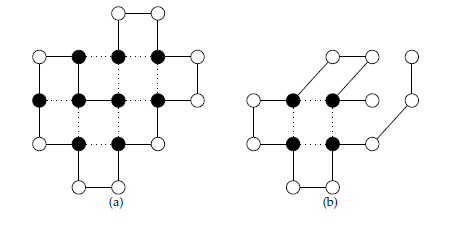
\includegraphics[scale=.8]{figuras/modeloHPExemplo.png}
			\caption{Exemplos de representação de proteínas utilizando os modelos HP 2D-HP (a) e 3D-HP (b). Fonte: Adaptado de \cite{santanna2008} }
			\label{fig:exemploModeloHP}
		\end{figure}

\end{frame}



\subsection{Representação do Problema}
\begin{frame}[allowframebreaks]{Representação do Problema}
	
	\begin{itemize}
		\item Existem várias maneiras de representar as conformações no modelo HP.
		\item 	Coordenadas relativas: O conjunto de movimentos possíveis para a grade 2D é definido por $\{F,E,D\}$, que correspondem aos movimentos: frente (continuar no mesmo sentido do aminoácido anterior), à esquerda e à direita. 
		\item Geralmente se utiliza uma codificação utilizando números inteiros, como por exemplo:  F$->$0, E$->$1 e D$->$2. 
	\end{itemize}
	
	\begin{figure}[!htb]
		\centering
		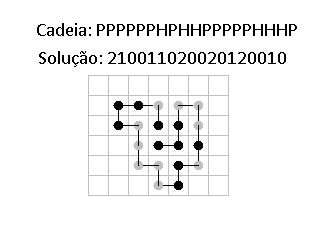
\includegraphics[scale=.8]{figuras/ExemploCodificacao.png}
		\caption{Exemplo de conformação gerada por uma solução codificada utilizando coordenadas relativas para uma cadeia de 20 aminoácidos.  Fonte: Autoria Própria }
		\label{fig:exemploCodificacao}
	\end{figure}



	
\end{frame}

	
